\section{Verifying calibration}
\label{sec:verifying_calibration}

\newcommand{\pluginEst}[0]{\ensuremath{\hat{E}_{\textup{pl}}^2}}
\newcommand{\cancelEst}[0]{\ensuremath{\hat{E}^2}}
\newcommand{\ltwoerror}[0]{\ensuremath{{\hat{E}^*}^2}}
\newcommand{\piSmallBound}[0]{\ensuremath{\frac{12}{n}\log{\frac{2B}{\delta}}}}

\tm{I wonder we should have subscript for $\cancelEst$. $\ensuremath{\hat{E}_{\textup{cxl}}^2}$? Sounds a bit verbose..}
Even if we use a recalibration method the actual calibration error may be lower or higher than the theory predicts. This is particularly true if the model is tested on a slightly different distribution that what it is trained on. Before deploying our model we would like to ensure that it has an acceptable calibration error.

In this section we show that we can efficiently estimate the calibration error of binned models, if the binning scheme is 2-well-balanced. Prior work typically estimates each term in the calibration error directly from samples~\cite{nguyen2015posterior, hendrycks2019anomaly, kuleshov2015calibrated, hendrycks2019pretraining}. (Cites) notice that this leads to a biased estimate, and propose an approximate correction term to reduce the bias. Our contribution is to show that while the naive estimator requires samples proportional to $B$ to estimate the calibration error, the improved estimator requires samples proportional to $\sqrt{B}$.

Concretely, suppose we are interested in checking if our model has calibration error $\leq \epsilon$ \pl{but this is not what we actually show due to $r$}. If the calibration error is $> \epsilon$, then with high probability we should output that it is not calibrated \pl{be more precise}. If the calibration error is $< r\epsilon$, where $0 < r < 1$ is a user-specified effect size, then with high probability we should output that the model is calibrated. Suppose we wish to measure the calibration error of a model $f : \mathcal{X} \to S$ where $S \subseteq [0, 1]$ and $|S| = B$. Suppose we get an evaluation set $T_n = \{(x_1, y_1), \dots, (x_n, y_n)\}$. Past work estimates the calibration error by directly estimating each term from samples:

\begin{restatable}[Plugin estimator]{definition}{pluginDfn}
\label{dfn:plugin-estimator}
\pl{English: define $\hat y_i$ to be the empirical average for the $i$-th score}
  Let $L_s$ denote the $y_j$ values where the model outputs $s$, given by $L_s = \{ y_j \; | \; (x_j, y_j) \in T_n\wedge f(x_j) = s \}$. \pl{background this}Let $\hat{p_s}$ be the estimated probability of $f$ outputting $s$:
\[ \hat{p_s} = \frac{|L_s|}{n} \]
Let $\hat y_i$ be the empirical average of $Y$ when the model outputs $s$:
\[ \hat{y_s} = \sum_{y \in L_s} \frac{y}{|L_s|} \] 

  The plugin estimate for the $\ell_2^2$ calibration error is \tm{$\ell^2$ calibration error sounds clearer}the weighted squared difference between $\hat{y_s}$ and $s$:
\[ \pluginEst{} = \sum_{s \in S} \hat{p_s} (s - \hat{y_s})^2 \]
\end{restatable}
\pl{can we just use $L^2$ for this whole paper?}

\cite{brocker2012empirical, ferro2012bias} observe that the plugin estimator is biased. They propose to subtract an approximation of the bias from the estimate:

\pl{this formula is a bit out of nowhere; saying 'debiasing' is helpful, but can you actually say the criteria more formally and declaratively?}
\begin{restatable}[Debiased estimator]{definition}{cancelingDfn}
The cancelling estimator for the $\ell_2^2$ error is:
\[ \hat{E}^2 = \sum_{i=1}^b \hat{p_i} \Big[ (s_i - \hat{y_i})^2 - \frac{\hat{y_i}(1 - \hat{y_i})}{\hat{p_i}n-1} \Big] \]
\end{restatable}

Our main result is that to check if the $\ell_2^2$ calibration error is $\leq \epsilon^2$, the plugin estimator requires $\widetilde{\Theta}(\frac{B}{\epsilon^2})$ samples (Theorem~\ref{thm:final-plugin}) while the debiased estimator requires $\widetilde{\Theta}(\frac{\sqrt{B}}{\epsilon^2})$ samples (Theorem~\ref{thm:final-ours}\tm{maybe some links issues here? Our theorem shouldn't be in section D, right?}): \tm{$\Theta$ notations --- see comments in the last theorem}

\begin{restatable}[Plugin bound]{theorem}{finalPlugin}\tm{Should this be a corollary instead of a theorem?}
\label{thm:final-plugin}
  Suppose \pl{use English} $\forall i.\;p_i \geq \frac{1}{2B}$ and $n = \widetilde{\Theta}(\frac{B}{\epsilon^2})$ ignoring $\log$ factors. Then the plugin estimator can check if ${E^*}^2 \leq \epsilon^2$ with failure probability $\delta$, and constant effect size $0 < r < 1$. 
\end{restatable}

\begin{restatable}[Cancelling bound]{theorem}{finalCanceling}
\label{thm:final-ours}
Suppose $\forall i.\;p_i \geq \frac{1}{2B}$ and $n = \widetilde{\Theta}(B+\frac{\sqrt{B}}{\epsilon^2})$ ignoring $\log$ factors.\tm{$\Theta(..)$ ignoring log factors sounds a quite non-standard way to say this .. First, it's unclear at the first sight why you need $\Theta$ but not $\Omega()$, second, I think often people would say $n = \widetilde{\Omega}(...)$ where $\widetilde{\Omega}$ hides log factors. Maybe you can use n gtrsim ... because gtrsim'd precise meaning could be a bit more flexible. (we don't see to have the package to support gtrsim lesssim)} Then the cancelling estimator can check if ${E^*}^2 \leq \epsilon^2$ with failure probability $\delta$ and constant $r$. 
\end{restatable}

The proof of both theorems is in Appendix~\ref{sec:verifying_calibration}. The idea is that for the plugin estimator each term in the sum has bias $1/n$. These biases accumulate, giving total bias $B/n$. The debiased estimator has much lower bias and the estimation variance cancels across bins---this intuition is captured in Lemma~\ref{lem:c3_bound} which requires careful conditioning to make this argument go through.

Another way of thinking about this is that the debiased estimator needs fewer samples to get near the true calibration error: for the plugin estimator if $n = \widetilde{\Theta}(\frac{B}{{E^*}^2})$ then $\frac{1}{2} {E^*}^2 \leq \pluginEst{} \leq \frac{3}{2} {E^*}^2$ but for the debiased estimator if $n = \widetilde{\Theta}(\frac{\sqrt{B}}{{E^*}^2})$ then $\frac{1}{2} {E^*}^2 \leq \cancelEst{} \leq \frac{3}{2}{E^*}^2$.

These bounds suggest that estimating calibration error can be the bottleneck, underscoring the importance of the estimation problem, since under suitable conditions the variance reduced calibrator can calibrate with $\widetilde{\Theta}(B + \frac{1}{\epsilon^2})$ samples but we need $\widetilde{\Theta}(B + \frac{\sqrt{B}}{\epsilon^2})$ samples to check if the error is $\leq \epsilon$.

\pl{provide a few sentences for proof sketch - at least the highlights - standard concentration or anything new? what's the hard part?}

\tm{To address the Percy's comment above, I think one choice would be to mention the canceling effect --- anyway it's in the name of your estimator. So explain the the estimate for each bin is unbiased, and then variance got cancelled. By contrast, the bias accumulates for plug-in estimator.}

Past work in meteorology has shown that the debiased estimator performs better in practice -- the main contribution of our work here is to show that the estimator also has an \emph{improved sample complexity}. However, in the Appendix, we run experiments on CIFAR-10, and show that for any desired calibration error, the cancelling estimator enables us to pick out models with a better mean-squared error. We recommend the use of this estimator.

% We ran experiments on CIFAR-10 and Imagenet to compare the practical performance of the cancelling estimator and the plugin estimator. We split the validation set \pl{how big?} into two chunks $C_1$ \pl{maybe give these more meaningful names with subscripts? anyway, put them behind macros} and $C_2$ \pl{what sizes}. We use $C_1$ to re-calibrate and discretize a trained model using $B = 100$ bins. For varying values of $n$, we sample $n$ points, with replacement, from $C_2$, and estimate the calibration error using the cancelling estimator and the plugin estimator. We then compute the squared deviation of these estimates from the calibration error measured on the entire chunk $C_2$. We repeat this 1,000 times to get the mean squared deviation and confidence intervals. The results are in Figure~\ref{fig:mse_estimators}. \pl{always say what the result is: Figure shows that...}
% In the Appendix, we include results for ImageNet, ablations on $B$, and we visualize the histogram of the deviations.

% \pl{say explicitly that we never say 'not calibrated'; there's a disconnect between the theory, which requires $r$ and $\epsilon$ and what we're doing here}

% We also run a multi-class calibration experiment on CIFAR-10 to show that our estimator allows us to select models with a better \pl{lower} Brier \pl{should we just say MSE everywhere? just be consistent since you defined MSE at the beginning} score subject to a given calibration constraint. As before, we split the validation set into $C_1$ and $C_2$. On $C_2$, we estimate the calibration error using the plugin and cancelling estimators and use 100 Bootstrap resamples to compute a 90\% upper confidence bound on the estimate. We compute the Brier scores and the upper bounds on the calibration error for $B = 10, 15, \cdots, 100$ and show the Pareto curve in Figure~\ref{fig:mse_vs_ce_estimators}. The results show that for any desired calibration error, the cancelling estimator enables us to pick out models with a better Brier score.

% \begin{figure}
%   \centering
%   \centering
%      \begin{subfigure}[b]{0.45\textwidth}
%          \centering
%          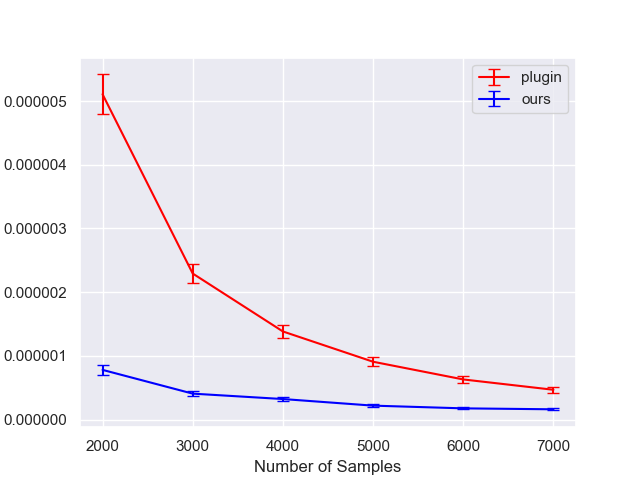
\includegraphics[width=\textwidth]{mse_estimator_100_bins.png}
%          \caption{Mean-squared errors of estimates.
%          \pl{s/ours/canceling}
%          \pl{Number of samples of what - relate to notation in text}
%          \pl{label y-axis}
%          }
%          \label{fig:mse_estimators}
%      \end{subfigure}
%      \hfill
%      \begin{subfigure}[b]{0.45\textwidth}
%          \centering
%          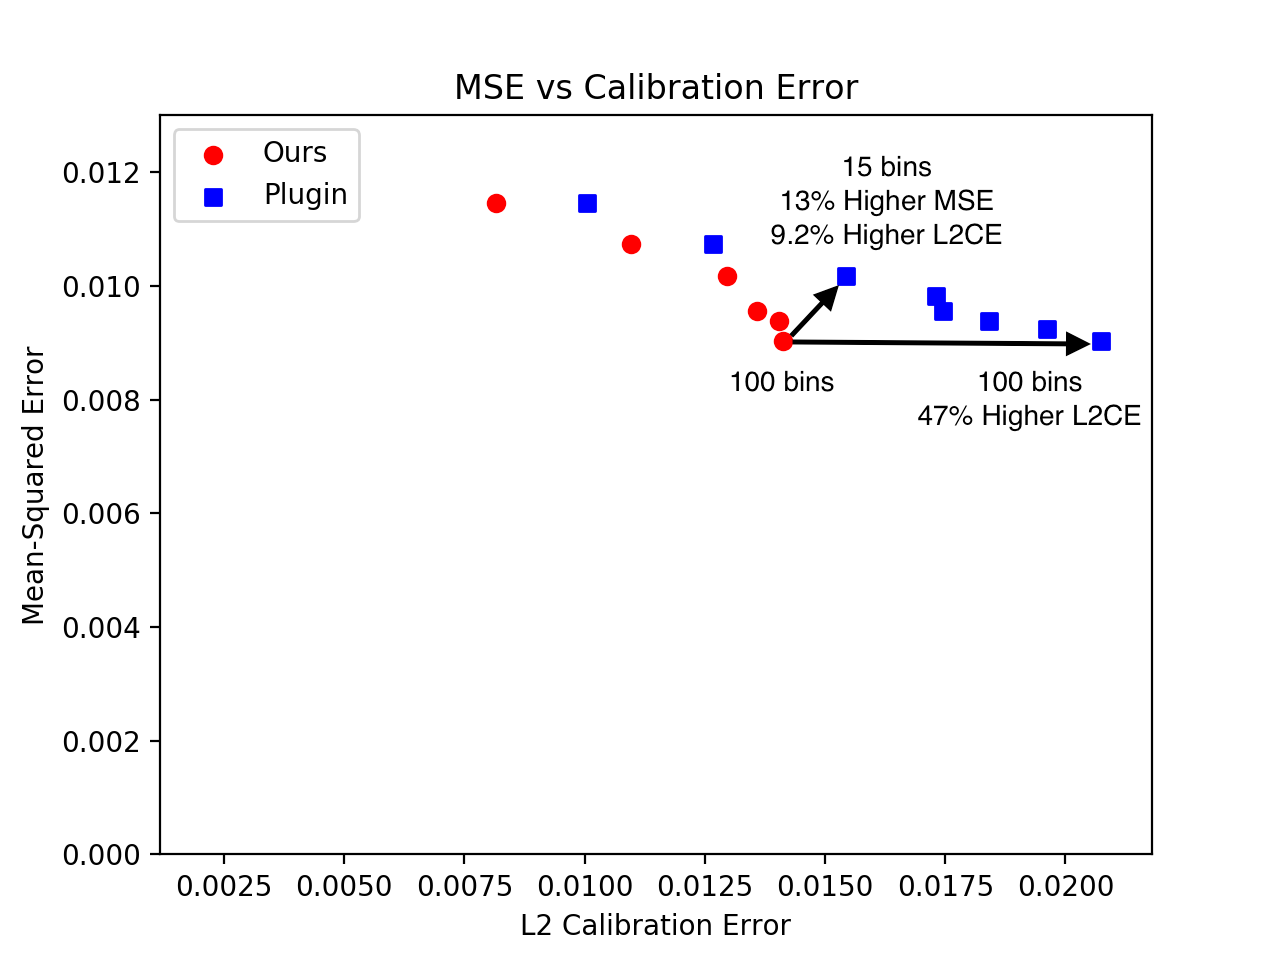
\includegraphics[width=\textwidth]{mse_vs_verified_error_plugin_vs_ours.png}
%          \caption{Brier score vs calibration error.
%          \pl{be consistent with MSE/Brier}
%          \pl{make text larger by reducing the xrange and yrange}
%          }
%          \label{fig:mse_vs_ce_estimators}
%      \end{subfigure}
%   \caption{
%     (\textbf{Left}) Mean-squared errors of cancelling and plugin estimators on a recalibrated VGG-net model on CIFAR-10 with $90\%$ confidence intervals (lower values better). Our estimator is closer to the ground truth \pl{what's ground truth? 0 on the y-axis?}.
%   (\textbf{Right}) Plot of Brier scores against upper bounds \pl{90\% confidence bounds or something?} on the calibration error computed by our estimator and the plugin estimator, when we vary the number of bins $B$. For a given calibration error, our estimator enables us to choose models with a better Brier score. If we want a model with $\ell_2$ calibration error less than 0.015, the cancelling estimator tells us we can confidently use 100 bins, while relying on the plugin estimator only lets us use 15 bins and incurs a 13\% higher Brier score.
%   \pl{I find it awkward that you have MSE (which is squared) plotted against calibration error (non-squared);
%   can we just make it RMSE instead?
%   }
% }
%   \label{fig:mse_estimators_bins}
% \end{figure}

% This means that our estimator has a substantially better dependency on the number of outputs of the model.

% \begin{corollary}
% \label{cor:final-ours}
% Using our estimator $\hat{E}$, if $n = \Theta(kb + \frac{\sqrt{b}}{\epsilon^2})$ ignoring $\log$ factors, we can check if $|{E^*} | \leq \epsilon$ with significance and power $\delta$, and constant effect size $r$. 
% \end{corollary}
